%%%%%%%% ICML 2021 EXAMPLE LATEX SUBMISSION FILE %%%%%%%%%%%%%%%%%

\documentclass{article}

% Recommended, but optional, packages for figures and better typesetting:
% \usepackage[english]{babel}
\newtheorem{lemma}{Lemma}
\newtheorem{theorem}{Theorem}
\usepackage{amsmath,amssymb,physics}
\usepackage{microtype}
\usepackage{graphicx}
\usepackage{subfigure}
\usepackage{booktabs} % for professional tables

% hyperref makes hyperlinks in the resulting PDF.
% If your build breaks (sometimes temporarily if a hyperlink spans a page)
% please comment out the following usepackage line and replace
% \usepackage{icml2021} with \usepackage[nohyperref]{icml2021} above.
\usepackage{hyperref}

% Attempt to make hyperref and algorithmic work together better:
\newcommand{\theHalgorithm}{\arabic{algorithm}}

% Use the following line for the initial blind version submitted for review:
% \usepackage{icml2021}

% If accepted, instead use the following line for the camera-ready submission:
\usepackage[accepted]{icml2021}

% The \icmltitle you define below is probably too long as a header.
% Therefore, a short form for the running title is supplied here:
\icmltitlerunning{Review on \textsc{Efficient Bandit Algorithms for Online Multiclass Prediction}}

\begin{document}

\twocolumn[
\icmltitle{Review on \textsc{Efficient Bandit Algorithms\\for Online Multiclass Prediction}}

% It is OKAY to include author information, even for blind
% submissions: the style file will automatically remove it for you
% unless you've provided the [accepted] option to the icml2021
% package.

% List of affiliations: The first argument should be a (short)
% identifier you will use later to specify author affiliations
% Academic affiliations should list Department, University, City, Region, Country
% Industry affiliations should list Company, City, Region, Country

% You can specify symbols, otherwise they are numbered in order.
% Ideally, you should not use this facility. Affiliations will be numbered
% in order of appearance and this is the preferred way.
% \icmlsetsymbol{equal}{*}

\begin{icmlauthorlist}
\icmlauthor{Xiaochen Zhu}{soc,math}     %{nus}%
% \icmlauthor{Author 2}{math}  %{nus}%
\end{icmlauthorlist}
    
\icmlaffiliation{math}{Department of Mathematics, National University of Singapore}
\icmlaffiliation{soc}{Department of Computer Science, National University of Singapore}
% \icmlaffiliation{nus}{National University of Singapore}
\icmlcorrespondingauthor{Xiaochen Zhu, A0194512H}{\texttt{xzhu@u.nus.edu}}
% \icmlcorrespondingauthor{Author 2}{email2@u.nus.edu}

% You may provide any keywords that you
% find helpful for describing your paper; these are used to populate
% the "keywords" metadata in the PDF but will not be shown in the document
\icmlkeywords{Machine Learning, ICML}

\vskip 0.3in
]

% this must go after the closing bracket ] following \twocolumn[ ...

% This command actually creates the footnote in the first column
% listing the affiliations and the copyright notice.
% The command takes one argument, which is text to display at the start of the footnote.
% The \icmlEqualContribution command is standard text for equal contribution.
% Remove it (just {}) if you do not need this facility.

%\printAffiliationsAndNotice{}  % leave blank if no need to mention equal contribution
\printAffiliationsAndNotice{} % otherwise use the standard text.

\begin{abstract}
    This report provides a critical review of the paper ``Efficient bandit algorithms for online multiclass prediction''\cite{kakade2008efficient}, which proposes an efficient algorithm, namely \textit{Banditron} for multiclass online learning with linear hypotheses in a bandit setting where the learner can only receive partial feedback about whether its prediction is correct or not, instead of the full information feedback which also contains the correct label. We review the Banditron algorithm and related proofs and discuss the positive points and contributions from an advocate perspective. Then, we identify some limitations with the algorithm, namely: (i) the mistake bound is polynomial to the number of examples; (ii) it is hard to optimally tune the hyperparameter $\gamma$. Then, we propose an improvement of Banditron to tackle the latter issue and theoretically show the mistake bound of the improved Banditron algorithm. At last, we address the incompleteness of our work (due to limited time) and further research work required to complement the current result.
\end{abstract}

\section{Overview}
\vspace{-.05in}

In convential multiclass machine learning (ML) settings, a learner aims to learn a model from a dataset $\mathcal{D}=\{(x_t,y_t):t\in\{1,2,\ldots,T\},x_t\in\mathbb{R}^d,y_t\in[k]=\{1,2,\ldots,k\}\}$ where $d$ is the dimension of examples and $k$ is the number of label classes. First, the learner initializes its model and make prediction $\hat{y_t}$ on example $x_t$. Then, it compares its own prediction $\hat{y_t}$ and the ground truth label $y_t$ to update its own model. However, in real world scenarios, one may not always have the privilege to know the actual labels but is only aware of the correctness of its predictions. We refer to this scenario as bandit setting, where the learner only has access to indicator $\mathbf{1}[\hat{y_t}=y_t]$ instead of $y_t$. Naturally, ML in bandit setting is an online (the learner cannot test a batch of examples at a time) multiclass (knowing $\mathbf{1}[\hat{y_t}=y_t]$ is equivalent to knowing $y_t$ for binary classification) classification problem, which has been extensively studied. The work of our interest, \citet{kakade2008efficient}, studies the learning of linear predicators in the bandit setting and proposes a variant of \textsc{Multiclass Perceptron} \cite{crammer2003ultraconservative}, namely \textsc{Banditron}. This section reviews the algorithm and gives a proof sketch on its mistake bound.
    
\subsection{Multiclass Perceptron}
Before introducing Banditron, we first discuss Multiclass Perceptron, the foundation of Banditron in the full information context (i.e. the learner receives ground truth labels $y_t$ instead of bandit feedback). In Multiclass Perceptron, the learner learns a model $W\in\mathbb{R}^{k\times d}$, where each row vector $W_j$ can be interpreted as a linear predictor $\theta_j\in\mathbb{R}^d$ as in the original binary Perceptron algorithm \cite{rosenblatt1958perceptron}. On example $\mathbf{x}_t,y_t$, the learner predicts $\text{argmax}_j (W\mathbf{x}_t)_j$, the index of the maximum prediction among all $\theta_j$ predictions. Similar to the binary Perceptron, Multicalss Perceptron updates $W$ on prediction mistakes, penalizing the row vector of $W$ making the wrong prediction and reinforcing the row vector of $W$ that should have given the greatest output. That is, given that $\hat{y_t}=\text{argmax}_j (W\mathbf{x}_t)_j$, then we have $\forall j\in[k]$,
\begin{equation}\label{eqn:perceptron_update}
    W^{(t+1)}_j=
    \begin{cases}
        W^{(t)}_j,&\text{if } \hat{y_t}=y_t\\
        \begin{cases}
            W^{(t)}_j - \mathbf{x}_t, &\text{if } j=\hat{y_t}\\
            W^{(t)}_j + \mathbf{x}_t, &\text{if } j=y_t
        \end{cases},&\text{if } \hat{y_t}\neq y_t
    \end{cases}
\end{equation}
Rearranging Equation (\ref{eqn:perceptron_update}), the update rule of Multiclass Perceptron can be expressed as $W^{(t+1)}=W^{(t)}+U^{(t)}$, where for all $j\in[k]$, \begin{equation}\label{eqn:perceptron_u}U^{(t)}_r=\mathbf{x}_t(\mathbf{1}[y_t=r]-\mathbf{1}[\hat{y_t}=r]).\end{equation}

Despite its simplicity, Multiclass Perceptron enjoys favorable mistake bounds. \citet{fink2006online} prove that if $\norm{\mathbf{x}_t}\leq1$ for all $t$, the number of mistakes (i.e. updates) Multiclass Perceptron makes to reach any fixed model $W^*\in\mathbb{R}^{(k\times d)}$ is upper bounded by $L+D+\sqrt{LD}$, where $L$ is the sum of hinge loss of $W^*$ on all examples \footnote{$L=\sum_{t=1}^T\max_{r\in[k]\setminus\{y_t\}}\max\{0,1-W^*_{y_t}\mathbf{x}_t+W^*_r\mathbf{x}_t\}$.} and $D=2\sum_{i=1}^{k}\sum_{j=1}^d (W^*_{ij})^2$, the \textit{complexity}\footnote{$D=2\norm{W^*}_F^2$, twice the square of Frobenius norm of $W^*$.} of $W^*$. Note that this bound is not assumed with any linear separability of $\mathcal{D}$. On contrast, \citet{crammer2003ultraconservative} shows that if $\norm{\mathbf{x}_t}\leq R$ for all $t$ and there exists a $W^*$ whose complexity $D\leq1$ that separate all examples correctly with a margin $\gamma$ (i.e. for all $t$, $W^*_{y_t}\mathbf{x}_t\geq\gamma/2$ and $W^*_i\mathbf{x}_t\leq\gamma/2$ for all $i\neq y_t$), the number of updates performed by Multiclass Perceptron is bounded by $2R/\gamma^2$. Since the focus of this review is Banditron, we will not prove these mistake bounds here.

\begin{algorithm}[bt]
    \caption{Banditron}\label{alg:band}
 \begin{algorithmic}
    \STATE \textbf{Given:} $\gamma\in(0,1)$
    \STATE Initialize $W^{(1)}\leftarrow\mathbf{0}\in\mathbb{R}^{(k\times d)}$
    \FOR{$t=1$ {\bfseries to} $T$}
    \STATE $\hat{y_t}\leftarrow\text{argmax}_j(W^{(t)}\mathbf{x}_t)_j$
    \STATE Choose from $\{\text{exploitation},\text{exploration}\}$ with probability $(1-\gamma,\gamma)$
    \IF{\text{exploitation}}
    \STATE $\tilde{y_t}=\hat{y_t}$
    \ELSE
    \STATE Randomly choose $\tilde{y_t}$ from $[k]$ uniformly
    \ENDIF
    \STATE $W^{(t+1)}\leftarrow W^{(t)}$
    \IF{$\tilde{y_t}\neq y_t$}
        \STATE Update $W^{(t+1)}_{\tilde{y_t}}\leftarrow W^{(t)}_{\tilde{y_t}}+\mathbf{x}_t/\text{P}(\tilde{y_t})$
        \STATE Update $W^{(t+1)}_{\hat{y_t}} \leftarrow W^{(t)}_{\hat{y_t}} - \mathbf{x}_t$
    \ELSE
    \STATE Update $W^{(t+1)}_{\hat{y_t}} \leftarrow W^{(t)}_{\hat{y_t}} - \mathbf{x}_t$
    \ENDIF
    \ENDFOR
 \end{algorithmic}
\end{algorithm}

\subsection{The Banditron algorithm}
Banditron, the main result of \citet{kakade2008efficient}, adopts the idea of Multiclass Perceptron. However, it cannot reinforce the row vector $W_{y_t}$ on mistakes because it does not receive ground truth labels $y_t$. Banditron addresses this issue by performing exploration rounds (predict based on a probability distribution) as well as exploitation rounds (predict based on its model $W$), which is a common idea in reinforcement learning. This is natural and intuitive because rather than being a supervised ML problem where the learner has access to a dataset with labels, the setting of ML with bandit feedback is more like reinforcement learning, where the learner has no information about the correct prediction, but only provided with a reward feedback on each of its actions, i.e. $\mathbf{1}[y_t=\hat{y_t}]$. The general idea of Banditron is that, on each example, the learner either explores with probability $\gamma$, where it randomly pick one label (i.e. each one with probability $\gamma/k$) to test, or explores with probability $1-\gamma$, where it predits $\hat{y}=\text{argmax}_j(W\mathbf{x}_t)_j$. Hence, on example $(\mathbf{x}_t,y_t)$, Banditron predicts $\hat{y_t}$ with probability $\gamma/k+1-\gamma$ and any other $i\neq\hat{y_t}$ with probability $\gamma/k$. Denote the probability of choosing $\tilde{y_t}=i$ as $\text{P}(i)$, the complete algorithm follows as Algorithm \ref{alg:band}. If one wants a closed-form update policy $W^{(t+1)}=W^{(t)}+\tilde{U}^{(t)}$ using the style of (\ref{eqn:perceptron_u}), we have for all $r\in[k]$ \begin{equation}\label{eqn:banditron_u}
    \tilde{U}^{(t)}_r=\mathbf{x}_t\left(\frac{\mathbf{1}[y_t=\tilde{y_t}]\mathbf{1}[r=\tilde{y_t}]}{\text{P}(r)}-\mathbf{1}[r=\hat{y_t}]\right).
\end{equation}

On correct predictions, if Banditron predicts by exploration, it reinforces the $\tilde{y_t}$-th row vector and penalize the $\hat{y_t}$-th row vector. If Banditron predicts correctly by exploitation, it adds $\mathbf{x}_t/\text{P}(\hat{y_t})-\mathbf{x}_t$ to the $\hat{y_t}$-th row vector which is an reinforcement since $1/\text{P}(\hat{y_t})>1$. On wrong predictions, Banditron subtracts $\mathbf{x}_t$ from the $\hat{y_t}$-th row vector, to make the algorithm \textit{unbiased} compared with Multiclass Perceptron, which is fomally defined in Lemma \ref{lem:unbias}.

\subsection{Mistake bound of Banditron}\label{sec:bound}
\citet{kakade2008efficient} proves a mistake bound similar to the $L+D+\sqrt{LD}$ bound for Multiclass Perceptron \cite{fink2006online}, stated in the following Theorem \ref{thm:bound}, whose concise sketch of proof will be discussed in this section.

\begin{theorem}[Mistake bound of Banditron]\label{thm:bound}
    If $\norm{\mathbf{x}_t}\leq1$ for all $t\in[T]$, then for any fixed model $W^*$, the number of mistakes $M$ made by Banditron satisifes \begin{equation}
        \mathbb{E}(M)\leq L+\gamma T+3\max\left\{\frac{kD}{\gamma},\sqrt{D\gamma T}\right\} + \sqrt{\frac{kDL}{\gamma}},
    \end{equation} where $L$ is the sum of hinge loss of $W^*$ on all examples and $D$ is the complexity of $W^*$ as defined earlier.
\end{theorem}

To bound the expectation of $M$, the number of mistakes Banditron makes when approaching $W^*$, naturally one investigates the term $\mathbb{E}[\langle W^*,W^{(t)}\rangle]$ \footnote{This is an extension of the conventionly inner product between vectors in the domain of matrices, i.e. $\langle A,B\rangle=\sum_i\sum_j A_{ij}B_{ij}$.}, which adopts the same idea used to prove the convergence bound of binary and multiclass Perceptron. The key ideas is to construct both an upper and a lower bound of $\langle W^*,W^{(t)}\rangle$. To do so, one needs the following lemmas, which can be proved by calculating the expectation w.r.t. $\tilde{y_t}$ using Equation (\ref{eqn:banditron_u}).

\begin{lemma}\label{lem:unbias}
    Banditron is unbiased compared with Multiclass Perceptron, in the sense for each update, that the expectation of Banditron's update matrix $\tilde{U}^{(t)}$ is the same as Multiclass Perceptron's update matrix $\tilde{U}$, w.r.t. the random variable $\tilde{y_t}$, that is, $\mathbb{E}_t[\tilde{U}^{(t)}]=U^{(t)}$.
\end{lemma}

\begin{lemma}\label{lem:frobenius}
    The expectation (w.r.t. $\tilde{y_t}$) of the squared Frobenius norm of $\tilde{U}^{(t)}$ is bounded as $\mathbb{E}_t[\Vert\tilde{U}^{(t)}\Vert^2_F]\leq2\norm{\mathbf{x}_t}^2\left(k/\gamma\mathbf{1}[y_t\neq \hat{y_t}]+\gamma\mathbf{1}[y_t=\hat{y_t}]\right)$.
\end{lemma}

First to lower bound $\mathbb{E}[\langle W^*,W^{(T+1)}\rangle]$, we have
\begin{equation}\label{eqn:5}
    \begin{aligned}
        &\mathbb{E}[\langle W^*,W^{(T+1)}\rangle]
        =\sum_{t=1}^T\mathbb{E}[\langle W^*,W^{(t+1)}\rangle]-\mathbb{E}[\langle W^*,W^{(t)}\rangle]\\
        &=\sum_{t=1}^T\mathbb{E}[\langle W^*,W^{(t+1)}-W^{(t)}\rangle]
        =\sum_{t=1}^T\mathbb{E}[\langle W^*,\tilde{U}^{(t)}\rangle]\\
        &=\sum_{t=1}^T\mathbb{E}[\langle W^*,U^{(t)}\rangle]\qquad\text{(by Lemma 1)}\\
        &\geq\sum_{t=1}^T\mathbb{E}[\mathbf{1}[\hat{y_t}\neq y_t]]-\ell_\text{hinge}(W^*,(\textbf{x}_t,y_t))
        =\mathbb{E}[\hat{M}]-L,
    \end{aligned}
\end{equation}
where $\hat{M}=\sum_{t=1}^T\mathbf{1}[\hat{y_t}\neq y_t]$. The last inequality is true because $\ell_{\text{hinge}}(W^*,(\mathbf{x}_t,y_t))\geq\mathbf{1}[\hat{y_t}\neq y_t]-\langle W^*,U^{(t)}\rangle$, derived from the definition of multiclass hinge loss.

Then, one wants to upper bound $\mathbb{E}[\langle W^*,W^{(T+1)}\rangle]$, using Cauchy-Schwartz and Jensen's inequalities, we have
\begin{equation}\label{eqn:6}
    \begin{aligned}
        &\mathbb{E}[\langle W^*,W^{(T+1)}\rangle]\leq\mathbb{E}[\Vert W^*\Vert_F\Vert W^{(T+1)}\Vert_F]\\
        &\leq\sqrt{\frac{D\mathbb{E}[\Vert W^{(T+1)}\Vert_F^2]}{2}}\qquad\text{(since }\sqrt{\cdotp}\text{ is concave)}.
    \end{aligned}
\end{equation}
Since $\Vert W^{(t+1)}\Vert_F^2=\Vert W^{(t )}\Vert_F^2+\langle W^{(t)},\tilde{U}^{(t)}\rangle+\Vert\tilde{U}^{(t)}\Vert^2_F$ for all $t\in [T]$, we then have
\begin{equation}\label{eqn:7}
    \begin{aligned}
        &\mathbb{E}[\Vert W^{(T+1)}\Vert_F^2]=\sum_{t=1}^T(\mathbb{E}[\langle W^{(t)},\tilde{U}^{(t)}\rangle]+\mathbb{E}[\Vert\tilde{U}^{(t)}\Vert^2_F])\\
        &=\sum_{t=1}^T(\mathbb{E}[\langle W^{(t)},{U}^{(t)}\rangle]+\mathbb{E}[\Vert\tilde{U}^{(t)}\Vert^2_F])\quad\text{(by Lemma 1)}\\
        &\leq\sum_{t=1}^T\mathbb{E}[\Vert\tilde{U}^{(t)}\Vert^2_F]\\
        &\leq\sum_{t=1}^T\mathbb{E}[\frac{2k}{\gamma}\mathbf{1}[y_t\neq \hat{y_t}]+2\gamma\mathbf{1}[y_t=\hat{y_t}]]\quad\text{(by Lemma 2)}\\
        &=\frac{2k}{\gamma}\mathbb{E}[\hat{M}] + 2\gamma T.
    \end{aligned}
\end{equation}

Substituting (\ref{eqn:7}) into (\ref{eqn:6}), we have
\begin{equation}\label{eqn:8}
    \begin{aligned}
    \mathbb{E}[\hat{M}]-L&\leq\mathbb{E}[\langle W^*,W^{(T+1)}\rangle]\\
    &\leq\sqrt{\frac{Dk\mathbb{E}[\hat{M}]}{\gamma}}+\sqrt{D\gamma T}.
    \end{aligned}
\end{equation}
Therefore, one can give an upper bound of $\mathbb{E}[\hat{M}]$ from (\ref{eqn:8}) and because Banditron explores no more than $\gamma T$ rounds, we have
\begin{align}
    &\mathbb{E}[M]\leq\mathbb{E}[\hat{M}]+\gamma T\label{eqn:9}\\
    &\leq L+\gamma T+3\max\left\{\frac{kD}{\gamma},\sqrt{D\gamma T}\right\} + \sqrt{\frac{kDL}{\gamma}}.\label{eqn:10}
\end{align}

\section{Contributions}\label{sec:positive}
\vspace{-.05in}
From the perspective of an advocate, this section discusses some of the contributions and positive points about \citet{kakade2008efficient}.
% \subsection{Mistake bound only dependent on $W^*$}

\subsection{As an unbiased variant of Multiclass Perceptron}
First of all, like its foundation Multiclass Perceptron, Banditron is an intuitive and simple algorithm that naturally makes sense. While Lemma \ref{lem:unbias} guarantees that the expected update matrix in Banditron is the same as Multiclass Perceptron, Banditron enjoys some of the advantages of Multiclass Perceptron such as the favorable performance (demonstrated in \citet{kakade2008efficient} empirically) and mistake bound (as proved in Section \ref{sec:bound}). As one of the earliest paper studying multiclass linear classification with bandit feedback, \citet{kakade2008efficient} enables further research to study this area more thoroughly. In short, the importance of the Banditron algorithm w.r.t. the bandit setting should be similar to that of the Perceptron \cite{rosenblatt1958perceptron} w.r.t. the full information setting.

\subsection{Mistake bound w.r.t. arbitrary $W^*$}\label{sec:2.2}
The approach \citet{kakade2008efficient} uses to provide a mistake bound for Banditron is similar to \citet{fink2006online}, which is given w.r.t. any fixed model matrix $W^*$ without any further assumptions on either the separability of $\mathcal{D}$ or the loss of $W^*$. In contrast, the mistake bounds for Perceptron and Multiclass Perceptron derived in \citet{rosenblatt1958perceptron,crammer2003ultraconservative} are made under the assumption of linear separability with a known margin and the existence of a zero-loss solution $W^*$. However, when running the algorithms, one cannot guarantee neither the existence of a solution nor the margin for linear separability, while the bounds in \citet{kakade2008efficient} and \citet{fink2006online} enables anyone to know the upper bound of mistakes when approaching any arbitrary goal $W^*$. Hence, the bound given by \citet{kakade2008efficient} is more generalized.

While it is not possible to derive the general case mistake boundary from the linear separable case, we can easily derive some mistake bound on the separable case from the general bound given by \citet{kakade2008efficient}. Assume that $\mathcal{D}$ is linearly separable and $W^*$ is a zero-loss solution, one can easily derive that $\mathbb{E}[M]$ is bounded by $O(\sqrt{T})$ by substituting $L=0$ in Equation (\ref{eqn:10}).

\section{Limitations}\label{sec:negative}
\vspace{-.05in}
From the perspective of a critic, this section discusses some of the limitations and negative points about the \citet{kakade2008efficient}.

\begin{figure}[t]
    \centering
    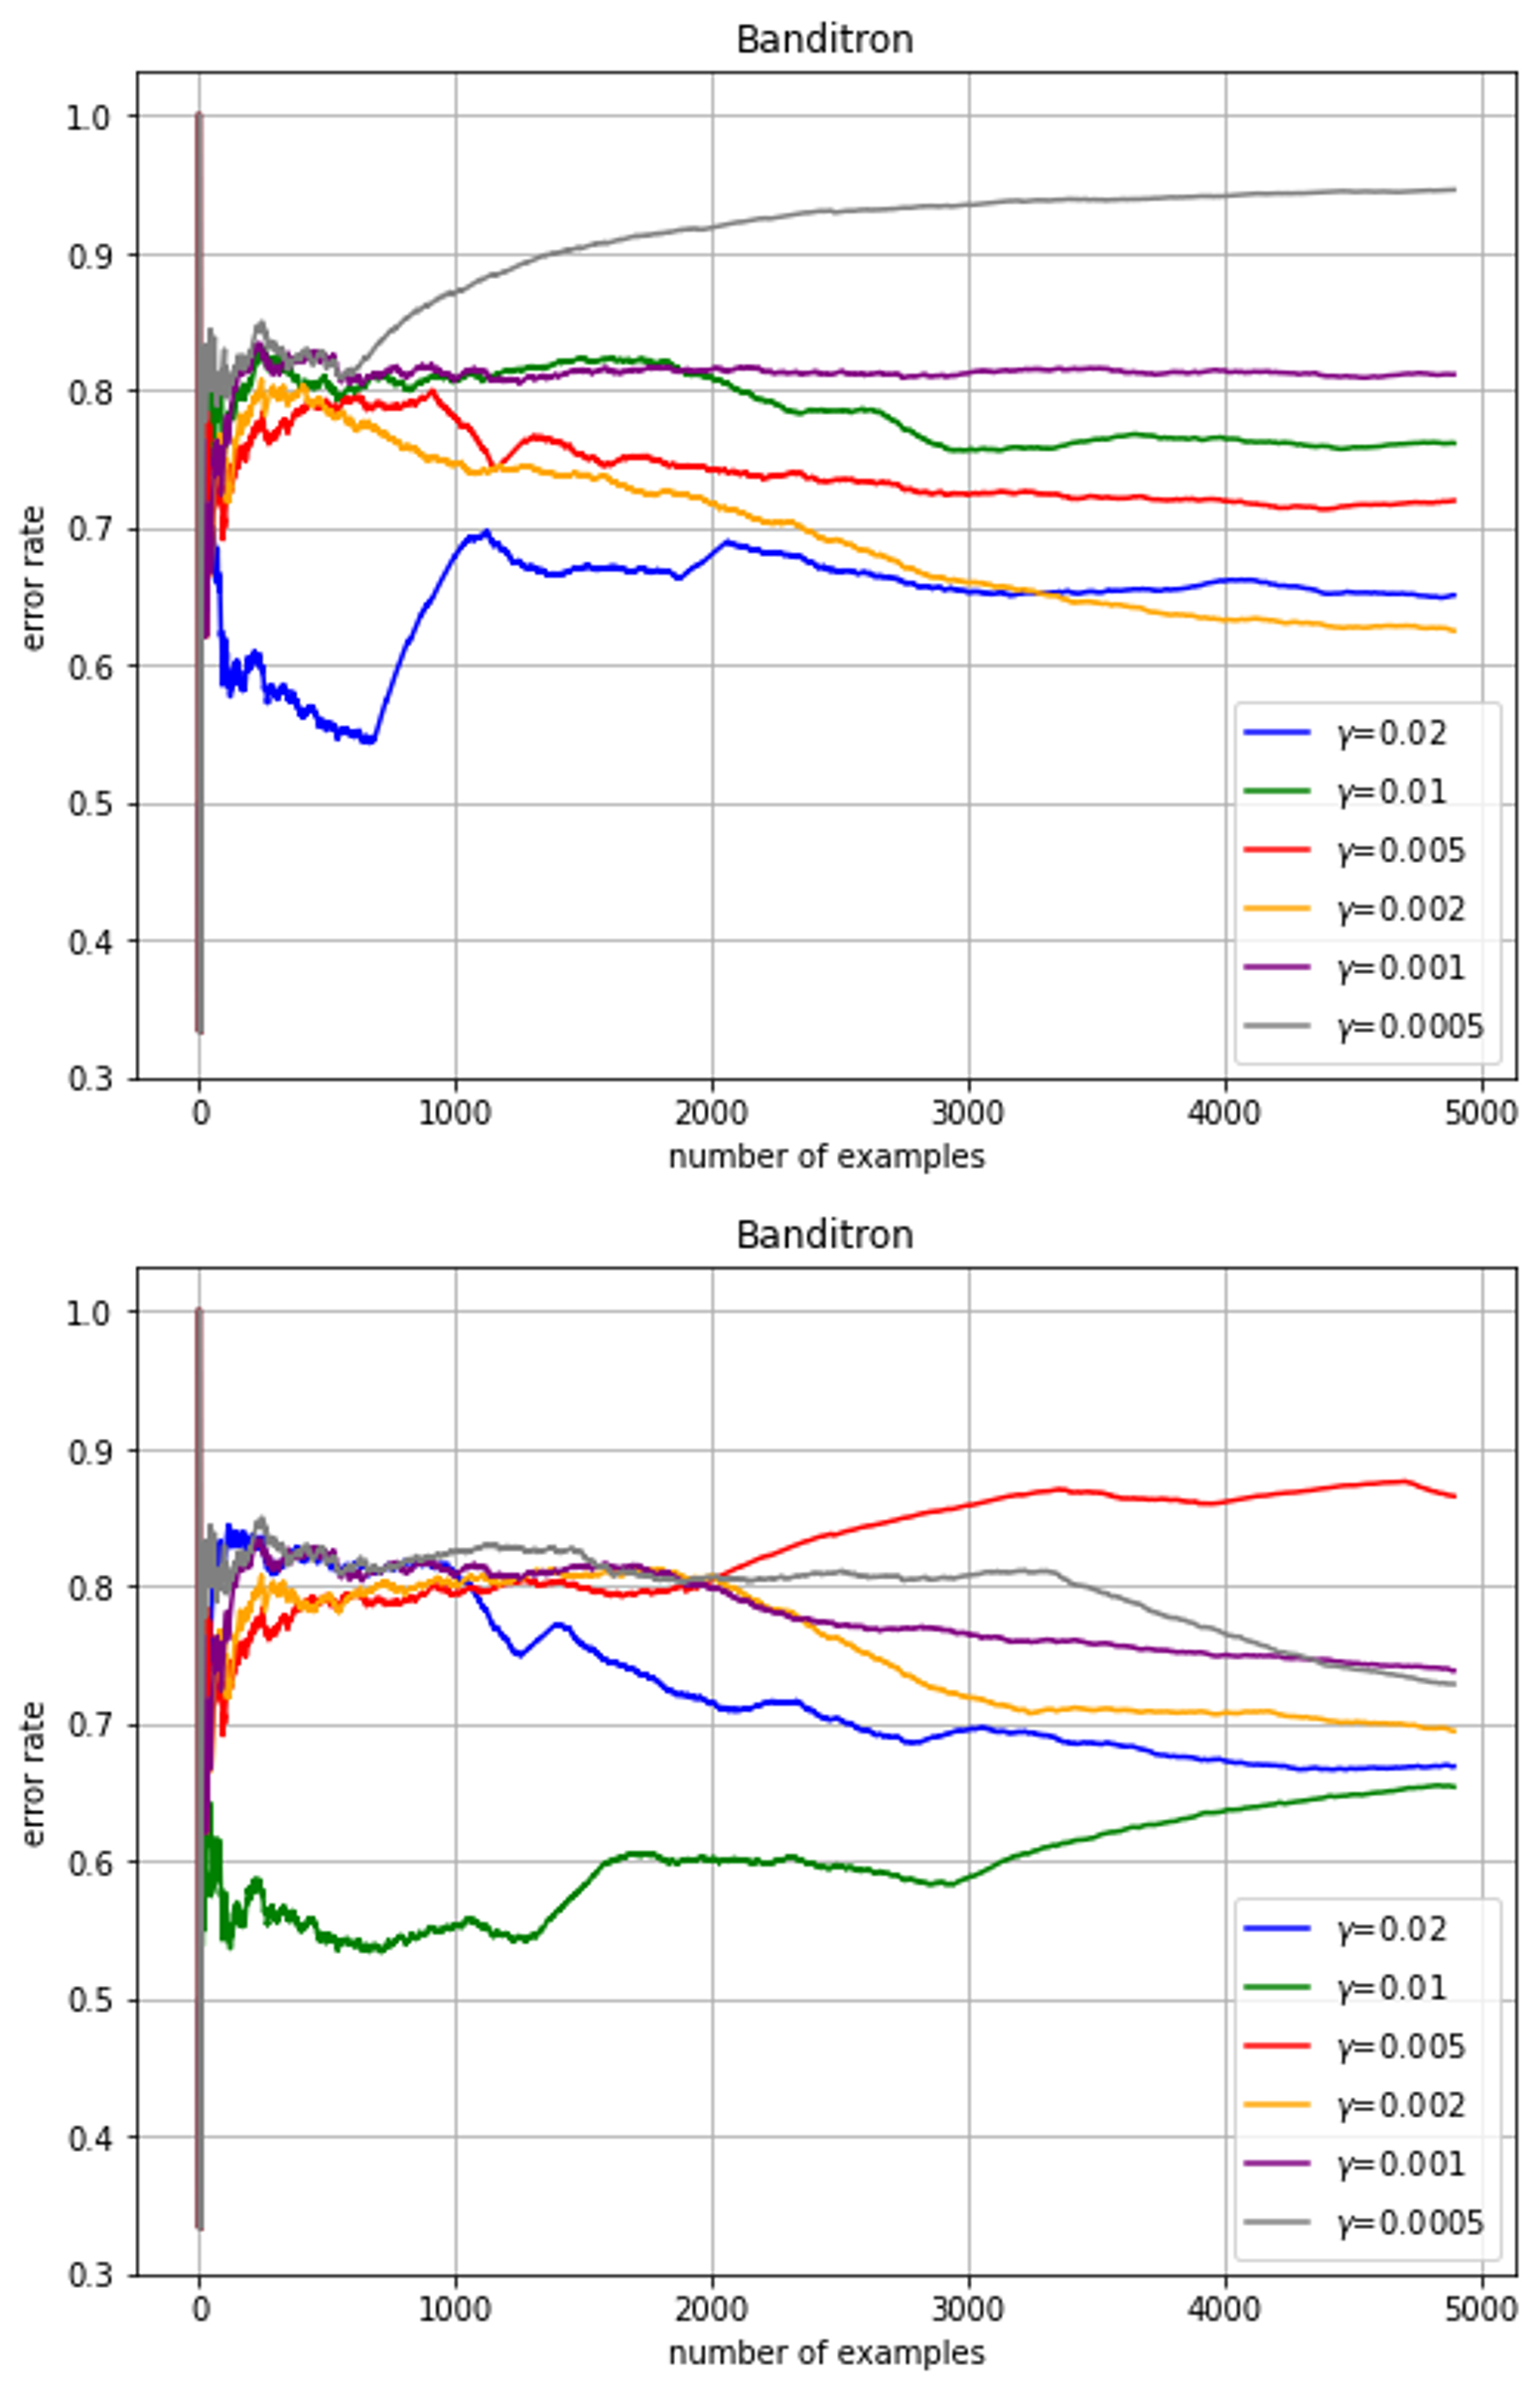
\includegraphics[width=0.7\linewidth]{./images/gammas.png}
    \label{fig:gammas}
    \caption{Two runs of Banditron with various $\gamma$}
\end{figure}

\subsection{Dependency of mistake bound on $T$}
Note that the mistake bound given by \citet{kakade2008efficient} (Theorem \ref{thm:bound}) is polynomial large w.r.t. the number of examples/updates $T$. Such dependency on $T$ does not exist on the mistake bounds in Multiclass Perceptron and has made Banditron's mistake bounds undesirable with a long time horizon. \citet{beygelzimer2019bandit} addresses this issue in the $m$-linearly separable case by proprosing an algorithm that achieve near-optimal mistake bound of $O(k/\sqrt{m})$.

\subsection{Tuning of hyperparameter $\gamma$}\label{sec:3.2}
Another limitation of Banditron is the difficulty in tuning of hyperparameter, namely the exploration-exploitation trade-off parameter $\gamma$. First, because of the randomness of the algorithm, the performance (i.e. error rate) of Banditron with different $\gamma$ values have high variation and can be dramastically different in each run. This has been demonstrated in Figure \ref{fig:gammas}, where the same algorithm with the same set of $\gamma$ values is executed on the dataset of Wine quality \cite{wine1999}, which is a non-linearly separable dataset with $k=7,d=11,T=4898$. We can see that different runs of the same parameter may result in dramastically different performance (i.e. in the first run, the best $\gamma$ seems to be $0.002$ while in the second run, the best $\gamma$ seems to be much larger at either $0.02$ or $0.01$). Even one can run the algorithm for multiple times and compare the average performance to choose $\gamma$, the high variantion of the performance will make such hyperparameter tuning less effective.

Another issue regarding tuning of $\gamma$ is that, the optimal $\gamma$ that can minimize error rate varies a lot on different datasets, the $\gamma$ chosen from the known dataset may not be applicable for predicting actual user behavior, while the learner cannot directly trains Banditron with user to with several $\gamma$ to choose the best one (because in bandit setting, the learner cannot choose the examples it sees or sees the same example over and over again, otherwise the learner can just trial and error every label until receiving a positive feedback). Hence, the choice of $\gamma$ seems to be difficult in real world applications.

\section{Extension}\label{sec:extension}
\vspace{-.05in}

\begin{algorithm}[bt]
    \caption{Banditron with variable $\gamma$}\label{alg:vari}
 \begin{algorithmic}
    \STATE \textbf{Given:} $\gamma_1,\gamma_2,\ldots,\gamma_T\in(0,1)$
    \STATE Initialize $W^{(1)}\leftarrow\mathbf{0}\in\mathbb{R}^{(k\times d)}$
    \FOR{$t=1$ {\bfseries to} $T$}
    \STATE $\hat{y_t}\leftarrow\text{argmax}_j(W^{(t)}\mathbf{x}_t)_j$
    \STATE $\gamma\leftarrow \gamma_t$
    \STATE Choose from $\{\text{exploitation},\text{exploration}\}$ with probability $(1-\gamma,\gamma)$
    \IF{\text{exploitation}}
    \STATE $\tilde{y_t}=\hat{y_t}$
    \ELSE
    \STATE Randomly choose $\tilde{y_t}$ from $[k]$ uniformly
    \ENDIF
    \STATE $W^{(t+1)}\leftarrow W^{(t)}$
    \IF{$\tilde{y_t}\neq y_t$}
        \STATE Update $W^{(t+1)}_{\tilde{y_t}}\leftarrow W^{(t)}_{\tilde{y_t}}+\mathbf{x}_t/\text{P}(\tilde{y_t})$
        \STATE Update $W^{(t+1)}_{\hat{y_t}} \leftarrow W^{(t)}_{\hat{y_t}} - \mathbf{x}_t$
    \ELSE
    \STATE Update $W^{(t+1)}_{\hat{y_t}} \leftarrow W^{(t)}_{\hat{y_t}} - \mathbf{x}_t$
    \ENDIF
    \ENDFOR
 \end{algorithmic}
\end{algorithm}

In this section, we introduce some extensions of Banditron theoretically and empirically, focusing on the use of variable $\gamma$ in Banditron. First, there are several issues with the constant $\gamma$ value in Banditron:
\begin{enumerate}
    \item As discussed in Section \ref{sec:3.2} constant $\gamma$ will have big impact on the performance and make it harder to tune;
    \item With constant $\gamma$, Banditron uses the same exploitation-exploration stategy even after a long time horizon, when the matrix $W$ should be able to reach a very small loss and Banditron should value exploitation more than exploration. Instead, Banditron still explores with probability $\gamma$. This is especially undesirable under separability.
\end{enumerate}

Motivated by these issues, we study the use of variable $\gamma$ instead of constant $\gamma$ in Banditron. If Banditron can still work under variable $\gamma$, then we can design better and more flexible update policies, such as exploration more in earlier iterations while exploitation more in later ones. Moreover, the sequence of $\gamma$ is potentially \textit{learnable} to minimize the error rate and therefore there's no need to tune the parameter.

The Banditron with variable $\gamma$ is given as Algorithm \ref{alg:vari}, and we can prove the following mistake bound for this algorithm.

\begin{theorem}[Banditron with variable $\gamma$]\label{thm:2}
    If $\Vert \mathbf{x}_t\Vert\leq1$ for all $t\in[T]$, then for any fixed model $W^*$, the number of mistakes $M$ made by Algorithm \ref{alg:vari} satisifes
    \begin{equation}
        \mathbb{E}[M]\leq L+\gamma_{\textup{sum}}+3\max\{\frac{kD}{\gamma_{\min}},\sqrt{D\gamma_{\textup{sum}}}\}+\sqrt{\frac{kDL}{\gamma_{\min}}}
    \end{equation} where $\gamma_{\min}=\min\{\gamma_1,\ldots,\gamma_T\},\gamma_{\textup{sum}}=\sum_{t=1}^T\gamma_t$ and $k,L,D$ have been defined previously.
\end{theorem}

We hereby provide a proof sketch of the stated theorem by modifying the original proof in Section \ref{sec:bound}.

First, note that although the $\gamma$ values in different rounds are different, the update policy in each round is still the same with the original Banditron of fixed $\gamma$. Therefore, Lemma \ref{lem:unbias} and \ref{lem:frobenius} are still true (other than replacing $\gamma$ with $\gamma_t$ in Lemma \ref{lem:frobenius}) given that the expectation is taken w.r.t. the choice of $\tilde{y_t}$ in a single round with one $\gamma$. Therefore Equation (\ref{eqn:5}) should still be true while Equation (\ref{eqn:7}) now becomes
\begin{equation}
    \begin{aligned}
        &\mathbb{E}[\Vert W^{(T+1)}\Vert_F^2]\\
        &\leq\sum_{t=1}^T\mathbb{E}[\frac{2k}{\gamma_t}\mathbf{1}[y_t\neq \hat{y_t}]+2\gamma_t\mathbf{1}[y_t=\hat{y_t}]]\quad\text{(by Lemma 2)}\\
        % &=\frac{2k}{\gamma}\mathbb{E}[\hat{M}] + 2\gamma T.
        &=\sum_{t=1}^T\mathbb{E}\left[\left(\frac{2k}{\gamma_t}-2\gamma_t\right)\mathbf{1}[y_t\neq\hat{y_t}]+2\gamma_t\right]\\
        &=2\gamma_{\text{sum}}+\sum_{t=1}^T\mathbb{E}\left[\left(\frac{2k}{\gamma_t}-2\gamma_t\right)\mathbf{1}[y_t\neq\hat{y_t}]\right]\\
        &\leq2\gamma_{\text{sum}}+\sum_{t=1}^T\mathbb{E}\left[\left(\frac{2k}{\gamma_{\min}}-2\gamma_{\min}\right)\mathbf{1}[y_t\neq\hat{y_t}]\right]\\
        % &=2\gamma_{\text{sum}}+\left(\frac{2k}{\gamma_{\min}}-2\gamma_{\min}\right)\mathbb{E}[\hat{M}]\\
        &\leq2\gamma_{\text{sum}}+\frac{2k}{\gamma_{\min}}\mathbb{E}[\hat{M}].
    \end{aligned}
\end{equation}

Therefore, similar to Equation (\ref{eqn:8}), we now have
\begin{equation}\label{eqn:13}
    \begin{aligned}
    \mathbb{E}[\hat{M}]-L&\leq\mathbb{E}[\langle W^*,W^{(T+1)}\rangle]\\
    &\leq\sqrt{\frac{Dk\mathbb{E}[\hat{M}]}{\gamma_{\min}}}+\sqrt{D\gamma_{\text{sum}}}.
    \end{aligned}
\end{equation}
Hence, one can derive an upper bound of $\mathbb{E}[\hat{M}]$ from Equation (\ref{eqn:13}). Since our algorithm in expectation runs $\gamma_{\text{sum}}$ exploration rounds, we have
\begin{equation}
    \begin{aligned}
    &\mathbb{E}[M]\leq \mathbb{E}[\hat{M}]+\gamma_{\text{sum}}\\
    &\leq L+\gamma_{\textup{sum}}+3\max\{\frac{kD}{\gamma_{\min}},\sqrt{D\gamma_{\textup{sum}}}\}+\sqrt{\frac{kDL}{\gamma_{\min}}}.
    \end{aligned}
\end{equation}

\section{Further research}
Therorem \ref{thm:2} enables Banditron to run with variable $\gamma$ values, which can be applied to design better update policies for Banditron. I have experimented several (intuitive) update policies on the datasets of wine quality and Iris \cite{wine1999,iris2019}, including:
\begin{itemize}
    \item a decreasing sequence of $\gamma$, preferring exploration first and then preferring exploitation in later rounds;
    \item adaptively modify $\gamma$ using the history accuracy of exploitation rounds and exploration rounds;
    \item set an initial $\gamma$ and a learning rate $\eta$, adaptively update $\gamma$ at each round by either $\gamma=\gamma+\eta$ or $\gamma=\gamma-\eta$, depending on the history performance of exploitation and exploration.
\end{itemize}

Unfortunately, none of these hypotheses consistently outperform the constant-$\gamma$ Banditron. However, we believe that Banditron with various $\gamma$ is still promising because it allows more flexibility than vanilla Banditron and introduces the possibility of automation (the algorithm adaptively updates its $\gamma$). Further research can be done to better study this area and propose working solutions to learn the variable $\gamma$ sequence.

% \section*{Acknowledgements}

% \newpage
% \vphantom{a} 
% \newpage
\bibliography{ref}
\bibliographystyle{icml2021}
    
    
%%%%%%%%%%%%%%%%%%%%%%%%%%%%%%%%%%%%%%%%%%%%%%%%%%%%%%%%%%%%%%%%%%%%%%%%%%%%%%%
%%%%%%%%%%%%%%%%%%%%%%%%%%%%%%%%%%%%%%%%%%%%%%%%%%%%%%%%%%%%%%%%%%%%%%%%%%%%%%%
% DELETE THIS PART. DO NOT PLACE CONTENT AFTER THE REFERENCES!
%%%%%%%%%%%%%%%%%%%%%%%%%%%%%%%%%%%%%%%%%%%%%%%%%%%%%%%%%%%%%%%%%%%%%%%%%%%%%%%
%%%%%%%%%%%%%%%%%%%%%%%%%%%%%%%%%%%%%%%%%%%%%%%%%%%%%%%%%%%%%%%%%%%%%%%%%%%%%%%
    
\end{document}
    
    
% This document was modified from the file originally made available by
% Pat Langley and Andrea Danyluk for ICML-2K. This version was created
% by Iain Murray in 2018, and modified by Alexandre Bouchard in
% 2019 and 2021. Previous contributors include Dan Roy, Lise Getoor and Tobias
% Scheffer, which was slightly modified from the 2010 version by
% Thorsten Joachims & Johannes Fuernkranz, slightly modified from the
% 2009 version by Kiri Wagstaff and Sam Roweis's 2008 version, which is
% slightly modified from Prasad Tadepalli's 2007 version which is a
% lightly changed version of the previous year's version by Andrew
% Moore, which was in turn edited from those of Kristian Kersting and
% Codrina Lauth. Alex Smola contributed to the algorithmic style files.